\documentclass{article}

\usepackage{hyperref}
\usepackage[T1]{fontenc}
\usepackage{graphicx}
\usepackage{float}
\usepackage[utf8]{inputenc}
\usepackage{amsmath}


\title{%
Laboratorium 9\\
  \huge Równania różniczkowe zwyczajne}
\author{Mateusz Król}
\date{22/05/2024 r.}

\begin{document}
\maketitle

 
\section*{Zadanie 1.}
\textbf{Przedstaw każde z poniższych równań różniczkowych zwyczajnych
jako równoważny układ równań pierwszego rzędu (ang. \textit{first-order system of ODEs}):\\\\
(a) równanie \textit{Van der Pol}'a:
$$y'' = y'(1-y^2) - y$$
(b) równanie \textit{Blasius}'a:
$$y''' = -yy''$$
(c) II zasada dynamiki \textit{Newton}'a dla problemu dwóch ciał:
$$y_1'' = -GM\cdot \frac{y_1}{(y_1^2+y_2^2)^{3/2}}$$
$$y_2'' = -GM\cdot \frac{y_2}{(y_1^2+y_2^2)^{3/2}}$$
}\\\\

Układy równań różniczkowych:\\
(a) równanie \textit{Van der Pol}'a:\\\\
Podstawienia:
    $$y_1=y$$
    $$y_2=y'$$
Układ równań:
    $$y_1'=y_2$$
    $$y_2'=y_2(1-y_2^2)$$
(b) równanie \textit{Blasius}'a:\\\\
Podstawienia:
    $$y_1=y$$
    $$y_2=y'$$
    $$y_3=y''$$
Układ równań:
    $$y_1'=y_2$$
    $$y_2'=y_3$$
    $$y_3'=-y_1y_3$$
(c) II zasada dynamiki \textit{Newton}'a dla problemu dwóch ciał:\\\\
Podstawienie:
    $$y_3=y_1'$$
    $$y_4=y_2'$$
Układ równań:
    $$y_1'=y_3$$
    $$y_2'=y_4$$
    $$y_3'=-GM\cdot \frac{y_1}{(y_1^2+y_2^2)^{3/2}}$$
    $$y_4'=-GM\cdot \frac{y_2}{(y_1^2+y_2^2)^{3/2}}$$

\section*{Zadanie 2.}
\textbf{Dane jest równanie różniczkowe zwyczajne
$$y'=-5y$$
z warunkiem początkowym $y(0) = 1$. Równanie rozwiązujemy numerycznie z
krokiem $h = 0.5$.
}\\\\

Poniższa tabela przedstawia wartości czynników amplifikacji dla zadanego
równania różniczkowego, dla każdej z omówionych metod.\\
Wartości te świadczą o numerycznej stabilności tych metod.

\begin{center}
  \begin{tabular}{c c} 
   Method & Amplification factor\\
   Explicit Euler & $-1.5$\\
   Implicit Euler & $\approx 0.286$\\
   Trapezoidal  & $\approx -0.111$\\
   Modified Euler & $1.625$\\
   RK4 & $\approx 0.648$
  \end{tabular}
\end{center}

Metody stabilne numerycznie dla zadanego równania to te, dla których
wartość bezwzględna z czynnika amplifikacji jest mniejsza od 1.\\
Są to metody: Implicit Euler, Trapezoidal, RK4.\\\\

Jawna metoda \textit{Euler}'a jest niestabilna numerycznie dla zadanego
parametru $h=0.5$.\\
Wzór iteracyjny:
$$y_{n+1} = y_n + h_n\lambda y_n$$
Wartość przybliżonego rozwiązania tą metodą dla $t=0.5$ wynosi
$y=-1.5$.\\

Wykres wartości rozwiązania wykorzystując jawną metodę \textit{Euler}'a:
\begin{figure}[H]
  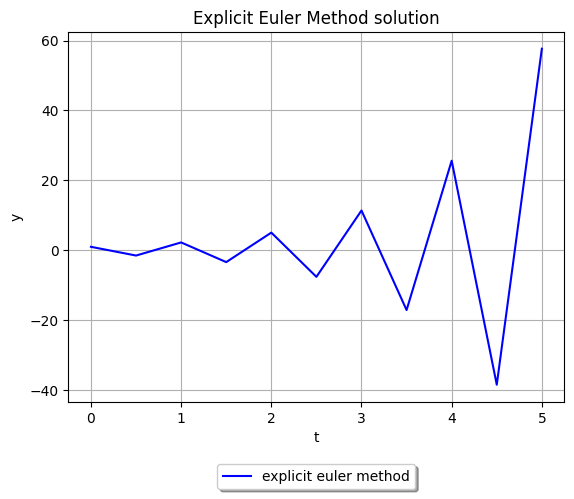
\includegraphics[width=\linewidth]{figures/explicit.png}
\end{figure}

Niejawna metoda \textit{Euler}'a jest stabilna numerycznie dla zadanego
parametru $h=0.5$.\\
Wzór iteracyjny:
$$y_{n+1} = \frac{y_n}{1 - h_n\lambda}$$
Wartość przybliżonego rozwiązania tą metodą dla $t=0.5$ wynosi
$y\approx 0.286$.\\

Wykres wartości rozwiązania wykorzystując niejawną metodę \textit{Euler}'a:
\begin{figure}[H]
  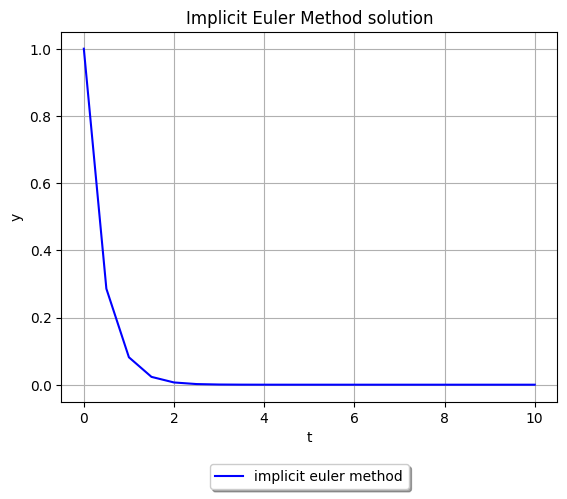
\includegraphics[width=\linewidth]{figures/implicit.png}
\end{figure}

\section*{Zadanie 3.}
\textbf{Model \textit{Kermack}’a-\textit{McKendrick}’a przebiegu epidemii w populacji
opisany jest układem równań różniczkowych:
$$S'=-\beta I S$$
$$I'=-\beta I S - \gamma I$$
$$R'=\gamma I$$
, gdzie: \\
S reprezentuje liczbę osób zdrowych, podatnych na zainfekowanie,\\
I reprezentuje liczbę osób zainfekowanych i roznoszących infekcję,\\
R reprezentuje liczbę osób ozdrowiałych.\\\\
Parametr $\beta$ reprezentuje współczynnik zakaźności (ang. \textit{transmission rate}).\\
Parametr $\gamma$ reprezentuje współczynnik wyzdrowień (ang. \textit{recovery rate}).\\
Wartość $\frac{1}{\gamma}$ reprezentuje średni czas choroby. \\\\
Założenia modelu:
\begin{figure}[H]
  \begin{itemize}
    \item Przyrost liczby osób zakażonych jest proporcjonalny do 
    liczby osób zakażonych oraz do liczby osób podatnych.\\
    \item Przyrost liczby osób odppornych lub zmarłych jest wprost proporcjonalny
    do liczby aktualnie chorych.\\
    \item Okres inkubacji choroby jest zaniedbywalnie krótki. \\
    \item Populacja jest wymieszana.
  \end{itemize}
\end{figure}
}



\end{document}